\chapter{Sign Language Learning Game in AR}

\section{Introduction}

Sign Language (SL) serves as the primary means of communication for individuals who are deaf or hard-of-hearing, utilizing visual movements to facilitate interaction with the world. However, the practice of SL requires a significant investment in learning, resulting in a communication gap between individuals who are mute and those who are able-bodied. According to the World Health Organization (WHO), as of 2020, the number of people affected by hearing disabilities was estimated at 466 million, including 34 million children \cite{el2020sign}. This number is projected to exceed 900 million by 2050.

In France alone, approximately 4 to 5 million individuals experienced difficulties or inability to communicate through speech due to hearing impairment in 2020. However, the exact figures for French Sign Language (LSF) users remain uncertain, with estimates ranging from 80,000 to 120,000, depending on the sources.

The human brain exhibits a natural affinity for learning through gestures, thanks to its innate mimicry reflex \cite{10.3389/fnhum.2012.00153}. Consequently, an effective learning solution should leverage this mimetic capability to guide learners in performing accurate gestures. With the advancements in augmented reality, the possibilities of dynamic and engaging learning experiences have significantly expanded. These techniques facilitate the acquisition of skills involving spatial movements through compelling visualizations.

Enhancing the learning process of SL can be achieved by fostering user engagement, surpassing the limitations of traditional methods such as watching sign language tutorial videos, utilizing apps, or attending lessons with an instructor. Augmented reality offers the potential to develop interactive characters that can effectively demonstrate gestures to learners. Combining such a program with gamification elements holds promise for promoting both user involvement and comprehension of movements.

The present work introduces a short video game designed for teaching sign language. While the application is intended to be used with the DVIC Interactive Mirror, it is fully functional on a standard personal computer as well.

The DVIC Augmented Mirror is a project developed with the goal of enabling the display of graphical elements overlaid onto the real environment as observed through the mirror glass. This device empowers users to monitor their own movements and compare them with a model, while also employing computer vision techniques to analyze the position of their limbs and verify the accuracy of performed gestures.

Consequently, the architecture of the learning game incorporates an artificial intelligence (AI) system for sign language recognition (SLR), utilizing the Mediapipe framework to extract the user's coordinates and analyzing them through a Pytorch-based model.

\subsection{GOSAI for Augmented Mirroir}

\subsubsection{GOSAI}

GOSAI \cite{gosai} is a new framework to help the development of augmented interfaces on the computer with a display. This framework targets all developers, from beginners to experts. GOSAI offers
basic and often used augmented reality functionalities. Thomas Juldo is a DVIC alumnus who developed the project, the augmented mirror system, and some applications. 

The system's structure allows it to reuse components between its applications and thus build a general catalog of tools that grows over time.

In addition, the framework uses mainstream programming languages to allow a wide range of developers to
use it. The framework is written in Python and Javascript.
Python is used for the framework's core components,
while Javascript is used for display.

JavaScript is a flexible programming language. It is one of the core
technologies of web development, and everyone can use it on both the
front-end and the back-end.
It is a versatile and robust language for video games. The developers can use JavaScript to make games using a variety of platforms and tools. They can use 2d and 3d libraries combined with JavaScript to create fully-fledged games in the browser or external game engine platforms \cite{javascriptgaming}.

\subsubsection{The interactive mirror}

The following projects presented in this thesis are implemented on an augmented mirror running on the GOSAI software system.

The augmented mirror is a platform that provides extensive interaction between the real and the virtual world. The objective is to create a recreational, medical, and educational platform.

A one-way mirror is placed against a screen. The mirror reflects perfectly where the screen is black and can display information when the pixels emit light. A camera is placed at the top of the mirror, facing slightly down. A laptop is placed at the back of the screen (see figure \ref{fig:mirror_062}).

\begin{figure}[h]
    \centering
    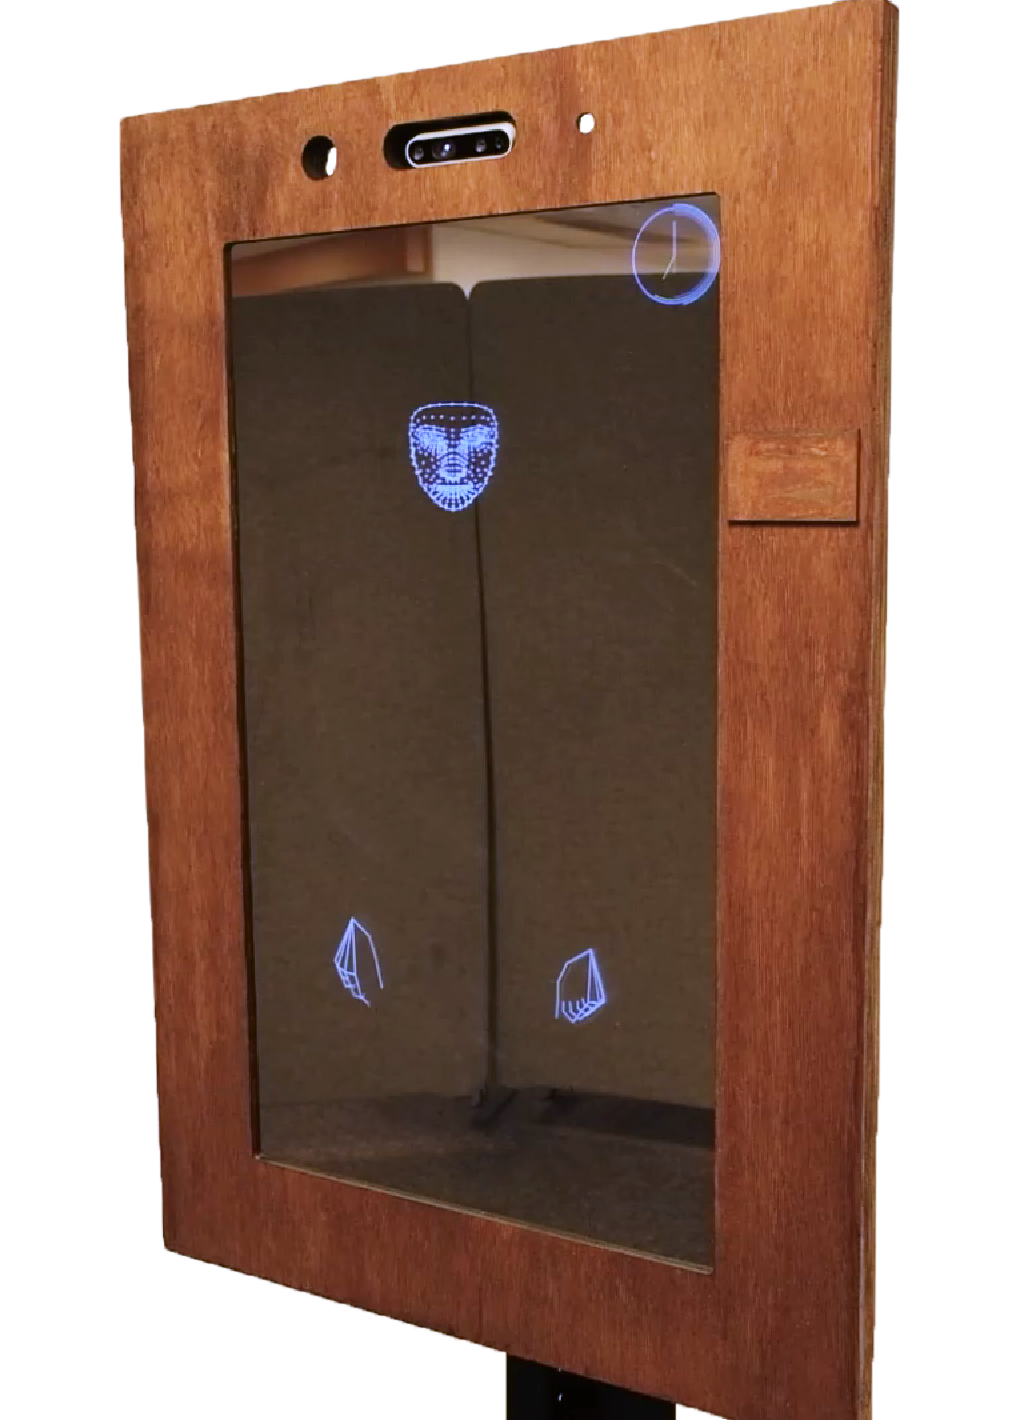
\includegraphics[width=0.9\columnwidth]{AdrLfv_master_thesis/images/mirror_062}
    \caption{The Augmented Mirror}
    \label{fig:mirror_062}
\end{figure}

% TODO resize l'image

The mirror can scan the room and detect and position objects the user interacts with. The augmented mirror uses the Intel D435 camera to estimate the position of a user in front of the mirror with Mediapipe. Thus, it can add a new dimension of interaction by exploiting kinesthesia. This dimension is an advantage over traditional interfaces using touch or a mouse. 

This interface is ideal for the development of applications requiring movement. It is relevant for the implementation of AI-assisted sign language learning modules.

\section{Related work}

\subsection{Sign Language Recognition}

A wide range of domains uses SLR for different purposes. It can be found in robotics, human services, games, virtual reality applications, direct or remote communication, or HCI projects \cite{adeyanju2021machine} (see figure \ref{fig:Polhemus}).

\begin{marginfigure}
    \centering
    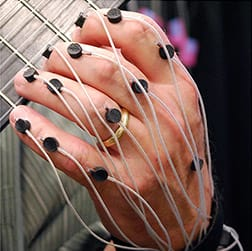
\includegraphics{AdrLfv_master_thesis/images/polhemus_tracker.jpg}
    \caption{Polhemus}
    \label{fig:Polhemus}
\end{marginfigure}

Many early SLR systems used data gloves and accelerometers to acquire specifics of the hands. The devices measure x,y,z, orientation, and velocity directly using a sensor such as the Polhemus tracker \cite{413199} \cite{5738842} or DataGlove \cite{Kadous1970} \cite{Metaxas1970} including accelerometers, gyroscopes, and electromyography sensors  (see figure \ref{fig:data_gloves}). Those techniques did not allow entire natural movement and constricted the mobility of the signer, altering the signs performed and being restrictive because of the need for supplementary material.

\begin{marginfigure}
    \centering
    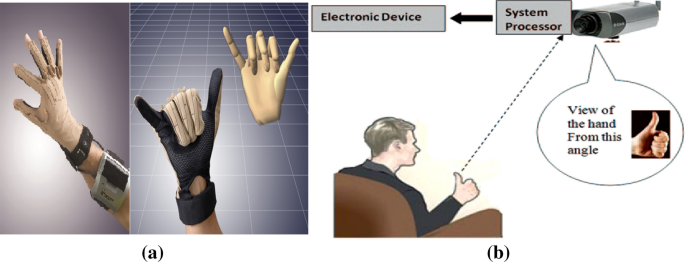
\includegraphics{AdrLfv_master_thesis/images/42979_2021_827_Fig3_HTML.png}
    \caption{Human–computer interaction using: a CyberGlove-II \cite{cyberglovesystems}, b vision-based system}
    \label{fig:data_gloves}
\end{marginfigure}

Most techniques based on data gloves convert the position of fingers and hands according to their angles into electrical signals to obtain the desired sign. 

In 2010, the ImageNet files appeared \cite{li2010crowdsourcing}. They provided a basis for the current CNNs and deep learning models, which was the beginning of computer vision. In 2012, AlexNet appeared and dramatically reduced the error rate for image recognition \cite{alom2018history}. After the appearance of these models, the use of data gloves is gradually abandoned to focus on the implementation of modules using computer vision.

Modern Computer vision-based techniques use pose estimation on the face, body, hands, and fingers to detect their position. This method uses images or videos of the signs through a camera and calculations on the images assisted by artificial intelligence \cite{adeyanju2021machine}. 

The identification of signs must take into account many different parameters. Facial expressions and body posture are vital in determining the meaning of sentences; e.g., eyebrow position can determine the question type. Some signs are distinguishable only by lip shape, as they share a common manual sign \cite{cooper2011sign}. 


\begin{marginfigure}
    \centering
    
    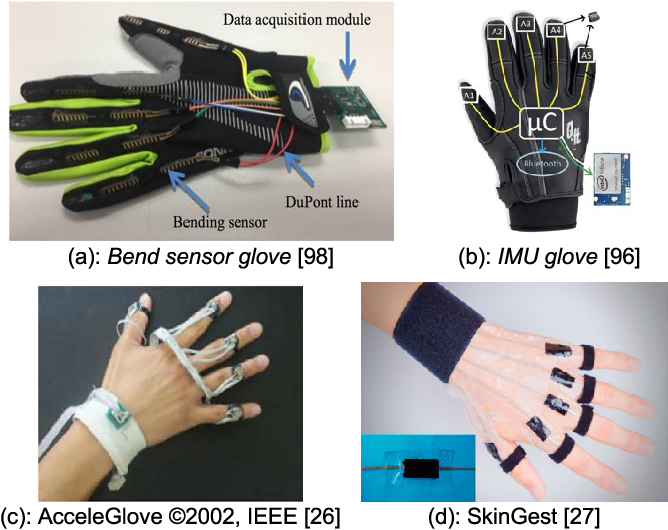
\includegraphics{AdrLfv_master_thesis/images/custom_gloves.png}
    \caption{Various custom gloves constructed by researchers in the sign language recognition field.}
    \label{fig:custom_gloves}
\end{marginfigure}

The speed of the sign realization can change the speed induced by the performed sign. A sign can also depend on its position on the body. All limbs must therefore be taken into account during the analysis. These challenges include sensor placement, data collection and preprocessing, and model training and evaluation \cite{9178440} (see figure \ref{fig:custom_gloves}).

Sign language recognition systems based on computer vision and wearable sensors have been proposed by several researchers \cite{ionescu2005dynamic} \cite{yu2010vision} \cite{li2015feature} \cite{sonkusare2015review} \cite{bobic2016hand} \cite{islam2017real} \cite{islam2017real} \cite{saha2018machine}, \cite{rastgoo2021hand} \cite{xu2021application}. 

\begin{marginfigure}
    \centering
    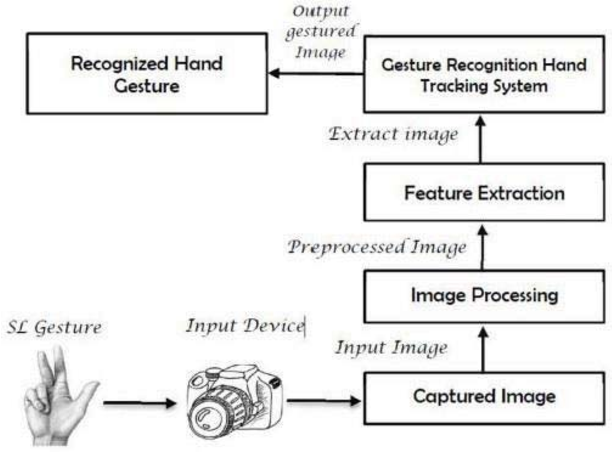
\includegraphics{AdrLfv_master_thesis/images/nimisha}
    \caption{Typical Vision Based Sign Language Recognition architecture.}
    \label{fig:nimisha}
\end{marginfigure}

Most recent SLR techniques use various image or vision-based SLR systems comprising feature extraction and classification \cite{nimisha2020brief} (see figure \ref{fig:nimisha}). 

Many projects using computer vision assisted SLR exist \cite{admasu2010ethiopian} \cite{deriche2019intelligent} \cite{ahram2021advances} \cite{song2021intelligent} \cite{lee2021american} \cite{lee2021comparative} \cite{gao2021rnn}. 

Many of these projects use a Convolutional Neural Network (CNN) model for predicting the American Sign Language (ASL) alphabet \cite{bin2019study}. Previously, classifiers like support vector machine \cite{savur2015real}, random forest, multilayer perceptron, transfer learning, and fine-tuning \cite{saleh2020arabic} were introduced for sign language recognition on simple images. Recently, shallow CNN and Capsule Networks have obtained better results \cite{hasan2020classification}. 

Skeleton coordinate-based action recognition with coordinates has recently been attracting more and more attention to compute sign language videos because of its invariance to the subject or background. In contrast, skeleton coordinate-based SLR only takes the crucial data for its learning. 

\begin{marginfigure}
    \centering
    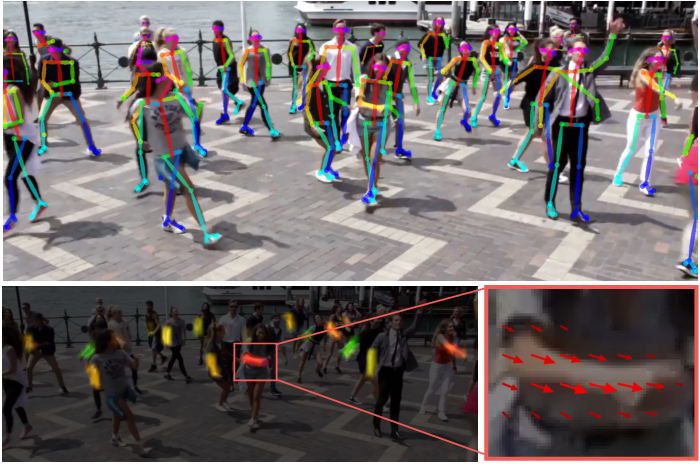
\includegraphics{AdrLfv_master_thesis/images/cao.png}
    \caption{Top: Multi-person pose estimation. Body parts of the same person are linked, including foot key points (big toes, small toes, and heels). Bottom left: Part Affinity Fields (PAFs) corresponding to the limb connecting the right elbow and wrist. The color encodes orientation. Bottom right: A 2D vector in each pixel of every PAF encodes the position and orientation of the limbs.}
    \label{fig:cao}
\end{marginfigure}

The most commonly used pose estimation frameworks that extract coordinates from a person using pose estimation are, for example, OpenPose \cite{cao2017realtime} (see figure \ref{fig:cao}), MoveNet \cite{movenet}, PoseNet \cite{kendall2015posenet} and MediaPipe \cite{lugaresi2019mediapipe}.



Techniques using computer vision or data gloves recover and process the coordinates with training methods. Various machine learning algorithms are used for sign language recognition, including neural networks, support vector machines, and hidden Markov models \cite{9178440}.

Adeyanju et al. comprehensively reviews the state-of-the-art techniques used in sign language recognition using machine learning \cite{almeida2014feature} \ref{fig:S0957417414003042}. The paper highlights the significance of sign language recognition and its potential to revolutionize communication between the deaf and hearing communities. The authors then review the different machine-learning techniques used for sign language recognition, such as Hidden Markov Models (HMMs), Support Vector Machines (SVMs), and Deep Neural Networks (DNNs).
The authors also highlight the importance of datasets in sign language recognition and review some of the commonly used datasets for sign language recognition. They emphasize the need for large, diverse datasets to train machine learning models effectively.

\begin{marginfigure}
    \centering
    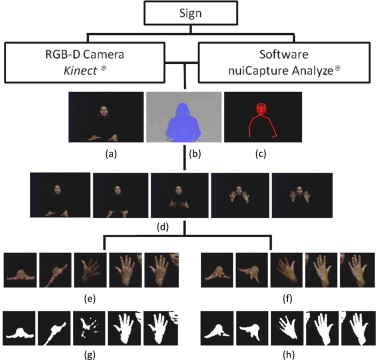
\includegraphics{AdrLfv_master_thesis/images/S0957417414003042.jpg}
    \caption{Feature extraction in Brazilian Sign Language Recognition based on phonological structure and using RGB-D sensors}
    \label{fig:S0957417414003042}
\end{marginfigure}

However, sign language is more than a collection of well-specified gestures.

%TODO ajouter le concours de google

\subsection{Sign Language Learning Video Games}

The video game is a dynamic audiovisual entertainment platform, accessible and stimulating the imagination of players. Using them to strengthen skills and abilities within society is possible. Video games are becoming increasingly valuable for children's development and youth culture.
They enhance the function of the attentional system, stimulate visual attention, reduce reaction time, and improve the ability to discriminate shape and color, plus efficiency when following multiple objects \cite{green2006enumeration}.

They are an efficient didactic way to promote interest and motivation by linking playfulness and pedagogical functions \cite{tejeiro2009efectos}.

The augmentation of interfaces thanks to technology, causes a better attractiveness of the learning method and thus an increase of the time voluntarily dedicated to self-learning and the motivation to concentrate on the method \cite{baker1994}.

Very few games use sign language as a primary element in the gameplay. We can cite Moss \cite{moss2018} (see figure \ref{fig:moss}), a video game on PlayStation VR in which the hero communicates with the player with ASL. 

\begin{marginfigure}
    \centering
    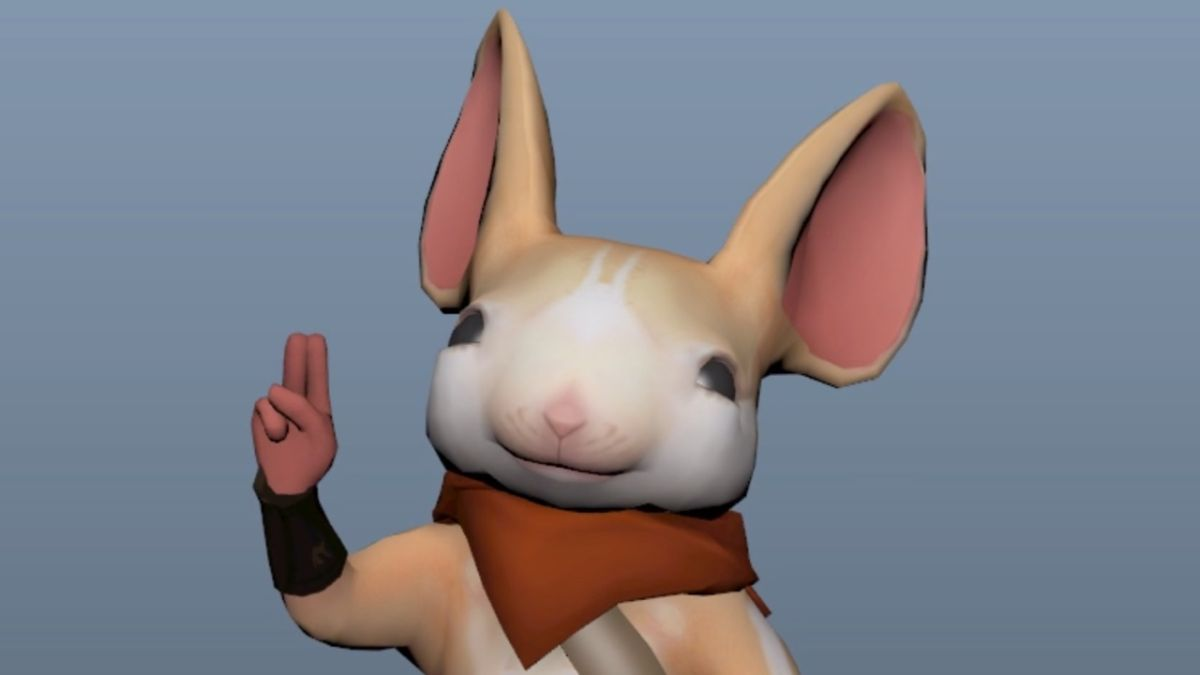
\includegraphics{AdrLfv_master_thesis/images/moss.jpg}
    \caption{Moss hero communicating with the player through American sign language}
    \label{fig:moss}
\end{marginfigure}

Zahoor Zafrulla et al. present Copycat, a game designed to improve the American Sign Language (ASL) skills of deaf children \cite{zafrulla2011copycat}. A team of researchers developed the game at the University of California in collaboration with members of the deaf community.
The game, called CopyCat, is a digital game that uses machine learning to provide feedback to the players. The game consists of a series of mini-games that focus on different aspects of ASL, such as finger spelling, vocabulary, and grammar (see figure \ref{fig:aslgamecopycat}). In each mini-game, the player watches a video clip of someone signing a word or phrase in ASL. The player is then asked to copy the sign or phrase using their signing.

CopyCat uses machine learning to analyze the player's signing and provide feedback on their performance. The authors designed the game to be adaptive, meaning it adjusts the difficulty level based on the player's skill level. The game also tracks the player's progress and provides feedback on improvement areas.
CopyCat developers then enhanced their SLR system with the Kinect depth-mapping camera, which uses colored gloves and embedded accelerometers to track children's hand movements \cite{zafrulla2011american}.

\begin{marginfigure}
    \centering
    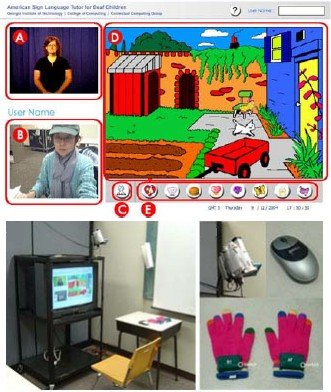
\includegraphics{AdrLfv_master_thesis/images/aslgamecopycat.jpeg}
    \caption{Screenshot of ASL Game Interface and the input devices for user  }
    \label{fig:aslgamecopycat}
\end{marginfigure}

\begin{marginfigure}
    \centering
    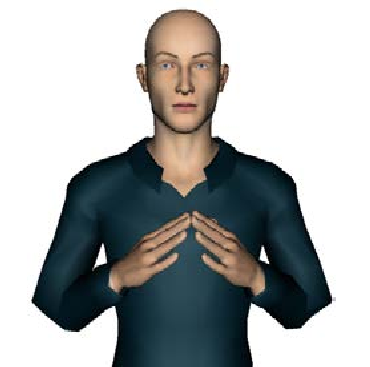
\includegraphics{AdrLfv_master_thesis/images/bouzid.png}
    \caption{The interpretation of the sign "house" via tuniSigner}
    \label{fig:bouzid}
\end{marginfigure}

Bouzid et al. explore using a learning game for SignWriting, a system for writing sign languages, to enhance sign language learning for students \cite{bouzid2016using}. The authors designed the game to be played on a computer or tablet. It includes various activities such as matching signs to their written symbols and translating written symbols into signs. The authors used a 3D human character to interpret the SignWriting notation. An avatar-based system called tuniSigner \cite{bouzid2013avatar} (see figure \ref{fig:bouzid}).

Lesmes et al. discuss the development of educational video games for deaf children in order to facilitate their inclusion in mainstream educational settings \cite{lesmes2022design}. 
The paper outlines the design and development process of educational video games, including using a participatory design approach that involves deaf children and educators throughout the design process. 
The authors designed the games to incorporate sign language, visual cues, and other features that would make them accessible to deaf children. The user can see an objective written on the left part of the interface, a character in the center, and an interpreter on the right (see figure \ref{fig:lesmes}).

\begin{marginfigure}
    \centering
    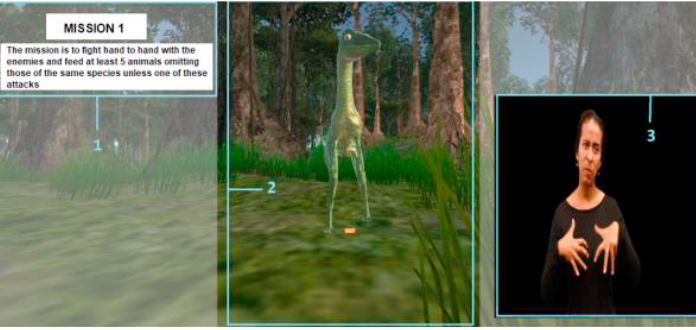
\includegraphics{AdrLfv_master_thesis/images/lesmes.png}
    \caption{Start interface of the videogame "Life of the Dinosaurs".}
    \label{fig:lesmes}
\end{marginfigure}

Most mobile applications for sign language learning are simple quizzes with a lesson and a questionnaire. PocketSign is an application for learning American Sign Language through interactive activities (see figure \ref{fig:pocketsign}). 
The project offers learning lessons, a dictionary for translating words into sign language videos, and a "fingerspelling" mode in which the user watches video tutorials of words or letters of the alphabet and then has to repeat them. 

\begin{marginfigure}
    \centering
    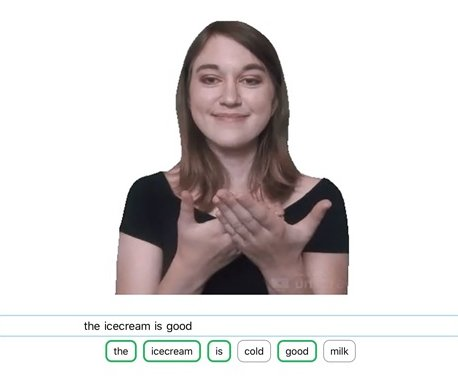
\includegraphics{AdrLfv_master_thesis/images/643x0w.jpg}
    \caption{example of exercise with a tutorial in Pocket Sign}
    \label{fig:pocketsign}
\end{marginfigure}

The application uses the phone's camera to film the user and verify that he or she is doing a word correctly before validating it and moving on to the next word.

\subsection{Visual Novel Engines}

\begin{marginfigure}
    \centering
    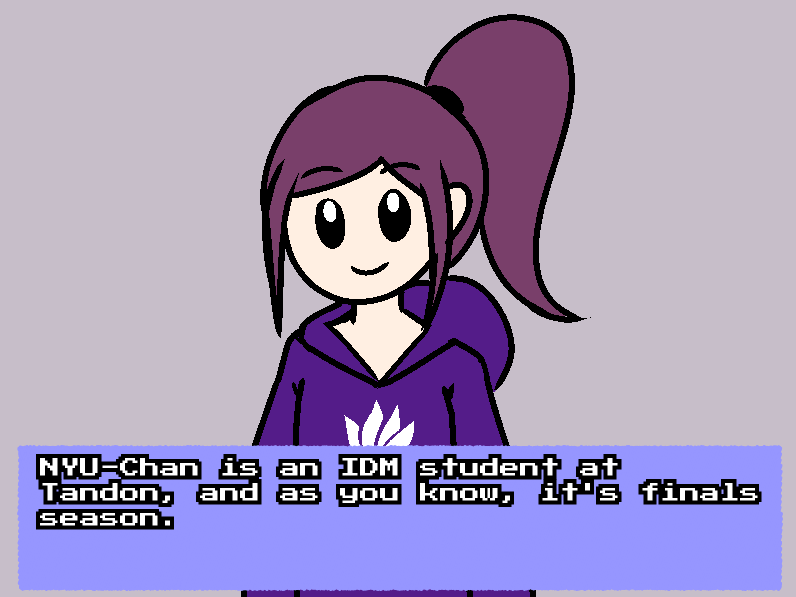
\includegraphics{AdrLfv_master_thesis/images/nyuchan.png}
    \caption{Presentation of the visual novel engine P5VN}
    \label{fig:nyuchan}
\end{marginfigure}

P5VN is an open-source Interactive Design and Media Major at NYU Tandon School of Engineering student project, allowing the creation of a visual novel using P5.js. It allows the display of dialogues, sprites, and backgrounds and using menus by clicking (see figure \ref{fig:nyuchan}). The game scenario is easily editable through a script that the engine parses. The project initially aimed to implement a prototype engine based on p5.js with a custom scripting language.  

Another visual novel engines, Tuesday JS \cite{TuesdayJS} or Monogatari \cite{monogatari} are simple web-based visual novel editors that can be used in a web browser. They are written in JavaScript, allowing the use of vector graphics svg, gif animations, and CSS styles.

Tuesay.js is an easy-to-use visual novel editor, free and open source. It runs on any web browser. The engine is written in JavaScript, does not use third-party libraries, and does not require additional software installation. It uses a drag-and-drop interface for editing scenes and creating interfaces. The script is displayed as a flowchart with all the elements and branches of the plot. The navigation is easy, and the editor helps to create stories with many plot options.

Monogatari.io is similar to Tuesday.js. The platform supports different media (images, videos, music) and multiple languages. It is highly customizable, open source, and multi-platform. 

JavaScript is a language adapted for the creation of projects like this one. 
The language is used extensively in games that only require a few resources. A 2D interactive game displays only a few details and elements.

Frameworks like Phaser JS library or p5.js are suitable for coding a simple game. p5.js is a JavaScript library for creative coding, focusing on making coding accessible and inclusive for artists, designers, educators, beginners, and anyone else. It can display graphics and process many different elements.

\subsection{Animated 3D Avatar}

\begin{marginfigure}
    \centering
    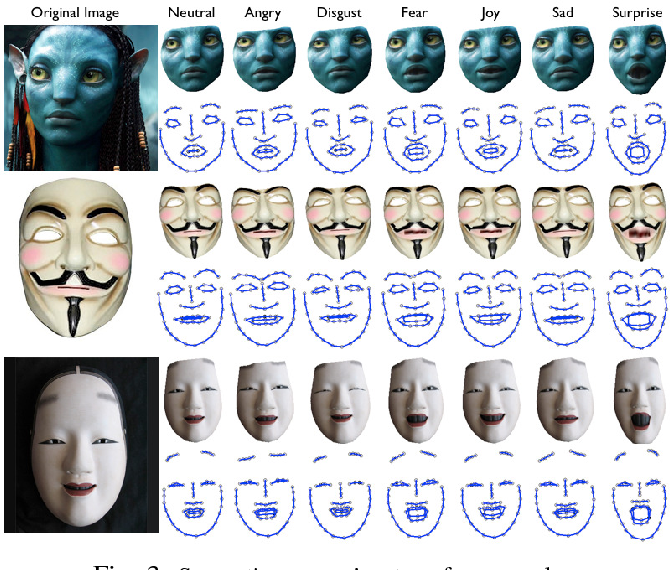
\includegraphics{AdrLfv_master_thesis/images/saragih.png}
    \caption{example of a real-time avatar animation from a single image thanks to semantic expression transfer.}
    \label{fig:saragih}
\end{marginfigure}

Most systems implement the display of an animated model from animation software (Blender, 3DS Max, Maya, Unity, Houdini) to create an animated avatar. The animations are worked directly in the software and then imported into a program for display in a game. 
Some projects allow the animation of a 3D model directly from the motion capture. In the project "Real-time Avatar Animation from a Single Image" \cite{saragih2011real} Saragih et Al. realize the modeling of 3D models from a simple photograph (see figure \ref{fig:saragih}). 

\begin{marginfigure}
    \centering
    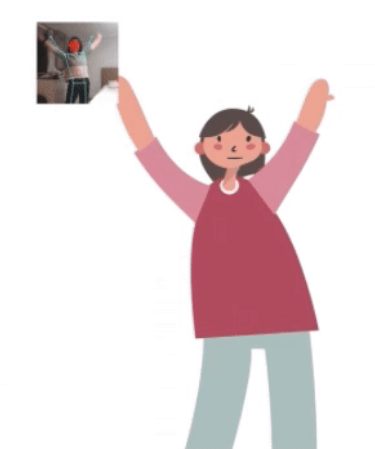
\includegraphics{AdrLfv_master_thesis/images/pose_animator.png}
    \caption{Animating full body character using FaceMesh and PoseNet with TensorFlow.js.}
    \label{fig:pose_animator}
\end{marginfigure}

A tool such as Unity or Maya can make its animation from MediaPipe coordinates. Pose Animator is a tool that gives rendering for 2D animation. A demonstration works with FaceMesh and PoseNet (from MediaPipe) online \cite{pose_animator} (see figure \ref{fig:pose_animator}). Unfortunately, this one does not understand the finger movements necessary for precise sign language tutorials.

\begin{marginfigure}
    \centering
    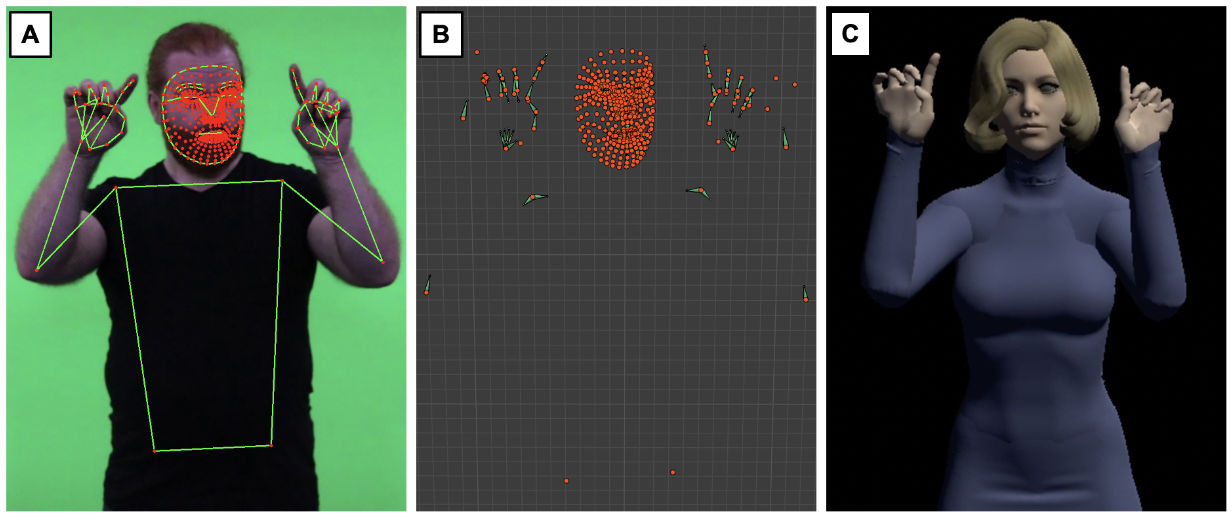
\includegraphics{AdrLfv_master_thesis/images/nguyen2021.png}
    \caption{Holistic tracking applied to a video frame. A) is the annotated original footage where
    the red dots are the tracked landmarks, while the green lines connect the joints. B) is the same
    frame in Blender with landmarks plotted as orange spheres and cyan-colored bones. C) shows the motion capture data applied to an avatar. \cite{nguyen2021automatic}}
    \label{fig:nguyen2021}
\end{marginfigure}

\begin{marginfigure}
    \centering
    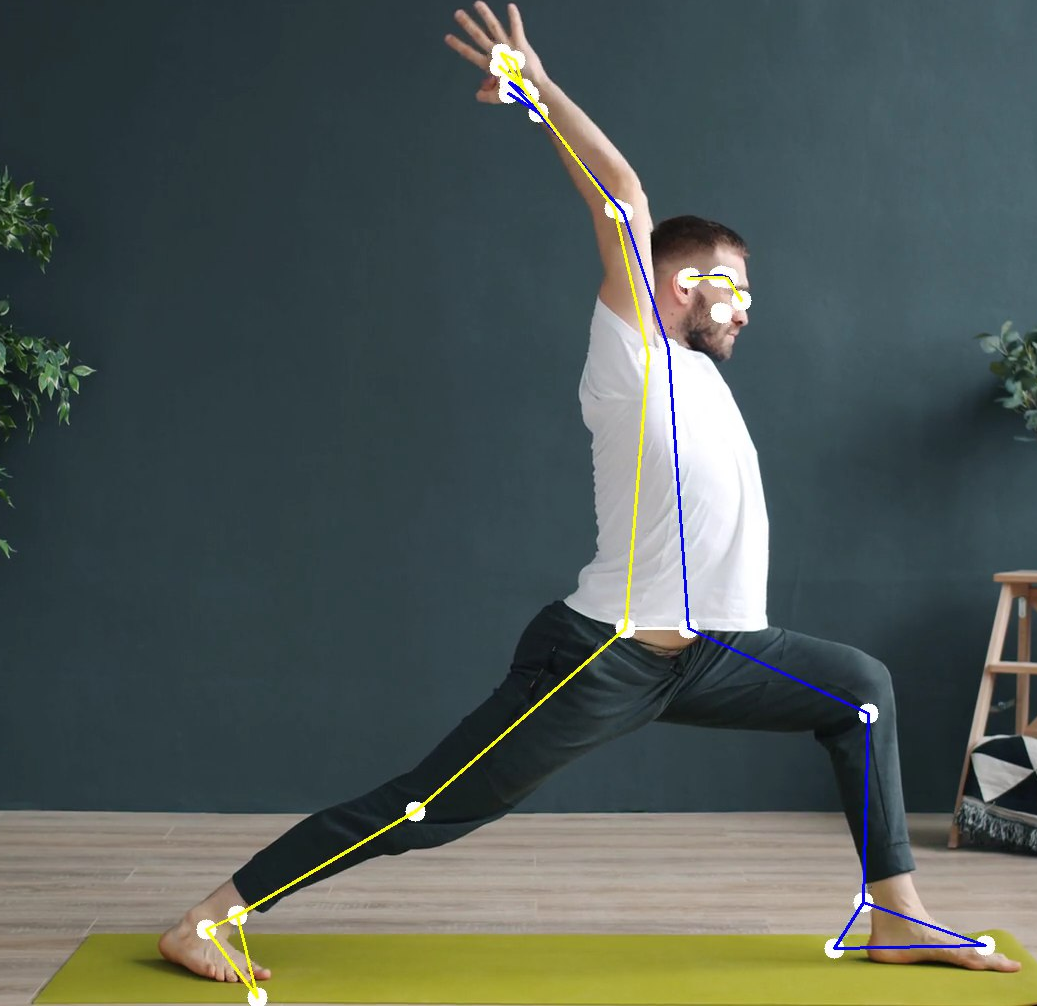
\includegraphics{AdrLfv_master_thesis/images/blazepose.png}
    \caption{BlazePose results on yoga use-cases}
    \label{fig:blazepose}
\end{marginfigure}

Another way is to adapt the coordinates in real-time to animate a character on Blender using Daz Studio as Nguyen et Al. \cite{nguyen2021automatic} (see \ref{fig:nguyen2021}). Most interactive avatars with pose estimation use MediaPipe and TensorFlow.js (namely FaceMesh, BlazePose, and HandPose) \cite{blazepose} (see \ref{fig:blazepose}).

\begin{marginfigure}
    \centering
    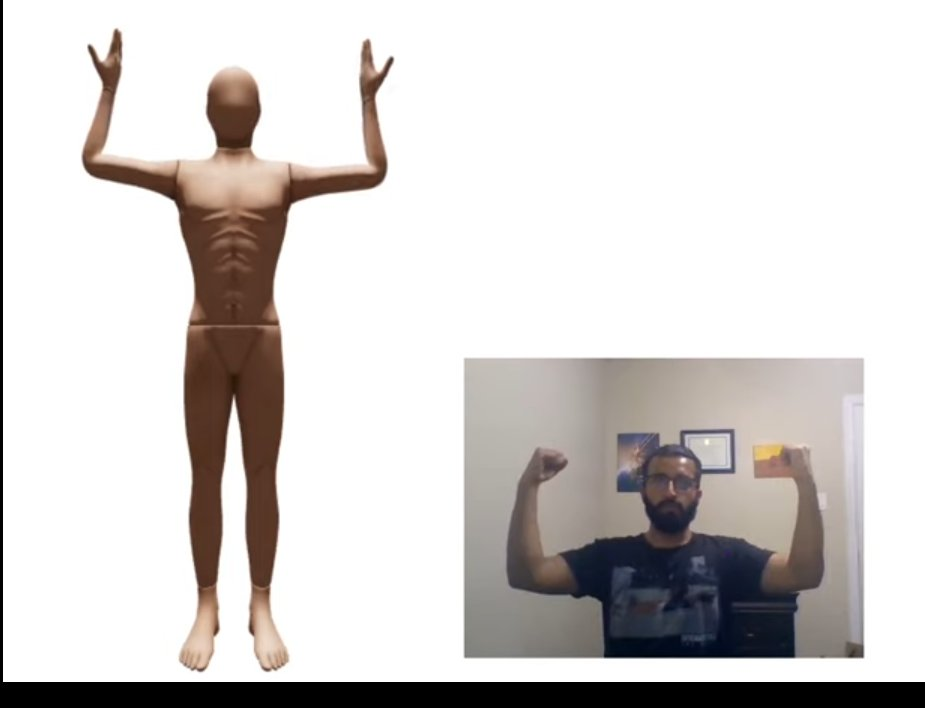
\includegraphics{AdrLfv_master_thesis/images/posenet_demo.jpg}
    \caption{React project that will allow us to move a 3D model with Three.js (React Three Fiber) and TensorFlow's Pose Estimation model (PoseNet).}
    \label{fig:posenet_demo}
\end{marginfigure}

Posenet\_demo \cite{posenet_demo} is a project allowing moving a 3D model with Three.js and Tensorflow's Pose Estimation model (PoseNet). The model uses Tensorflow and PoseNet to detect the critical points of the joints in each frame and then send those points over to the Model file. 

The project uses an Adobe Mixamo \cite{mixamo} 3D model in FBX format and Blender to import the FBX format and export a GLB format \cite{posenet}. The avatar follows the head and shoulder's inclination (see \ref{fig:posenet_demo}).

A last interesting example is that of Kalidokit \cite{kalidokit}. Kalidokit is a tool that uses Mediapipe\/Tensorflow.js models for tracking face, eyes, pose, and hand movements.
It is compatible with various models such as Facemesh, Blazepose, Handpose, and Holistic. The tool calculates simple Euler rotations and blendshape face values based on the predicted 3D landmarks.

\begin{marginfigure}
    \centering
    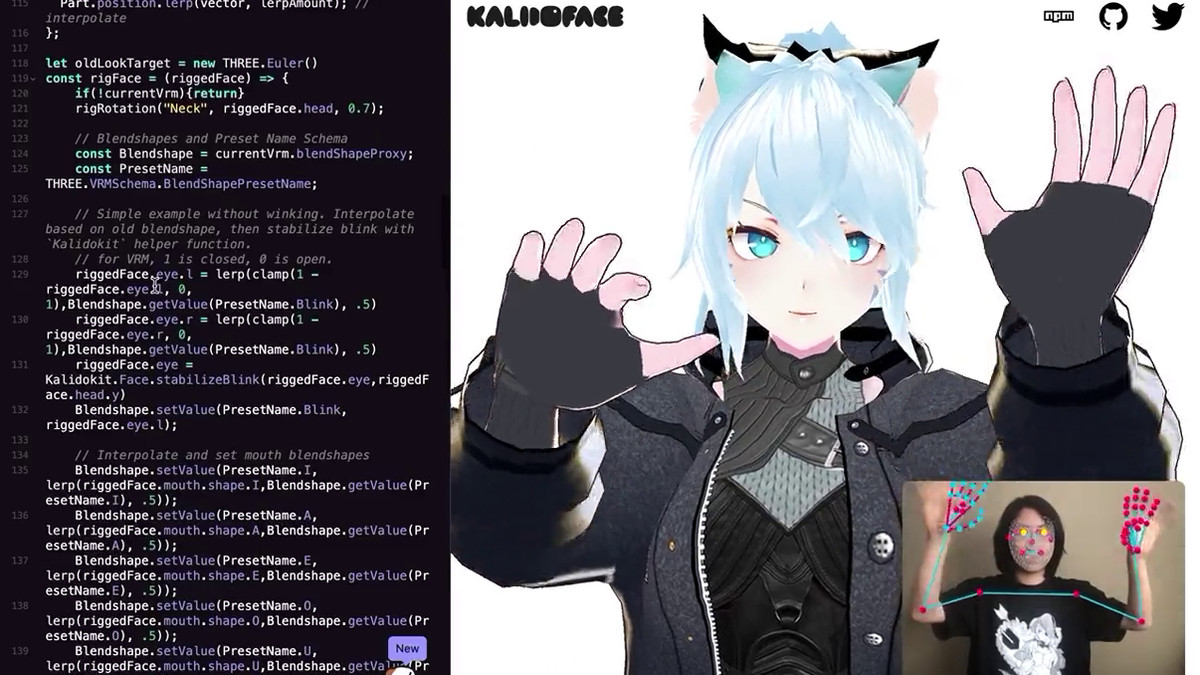
\includegraphics{AdrLfv_master_thesis/images/kalidoface.jpg}
    \caption{KalidoKit can move 3D avatars by tracking face and body movement with a simple webcam.}
    \label{fig:kalidoface}
\end{marginfigure}

Kalidokit is the core component for Vtuber web apps, such as Kalidoface and Kalidoface 3D. Its purpose is to rig 3D VRM models and Live2D avatars. The project is a JS library intended for developers using Mediapipe pre-trained models rather than a complete app. The library still has to be adapted to run on different platforms. The project is based on Three.js, a powerful library for creating three-dimensional models and games. 
With few lines of JavaScript, Kalidokit allows the creation of simple 3D patterns for photorealistic, real-time scenes. The library can create complex 3D geometrics and animate and move objects.

Three.js is a JavaScript library for creating 3D scenes in a web browser. It can be used with the HTML5 canvas tag without needing a plugin. The library enables the application of textures and materials. It also provides various light sources to illuminate scenes, advanced postprocessing effects, custom shaders, and load objects from 3D modeling software. It is easy to use, intuitive, and a well-documented library.

\section{Gameplay}

The sign language game is an augmented reality game, a visual novel on the augmented mirror. We follow a character during a short adventure where the user can make choices by making American Sign Language signs in front of the mirror. He can answer the characters, interact with objects, choose actions, and choose a path. 
Sometimes the player sees the tutorial of one, two, or three signs simultaneously. The user must then make the sign of the choice he takes. For example, he can turn right or left by making the appropriate sign (see \ref{fig:sleg_left_right}). 

\begin{figure}[h]
    \centering
    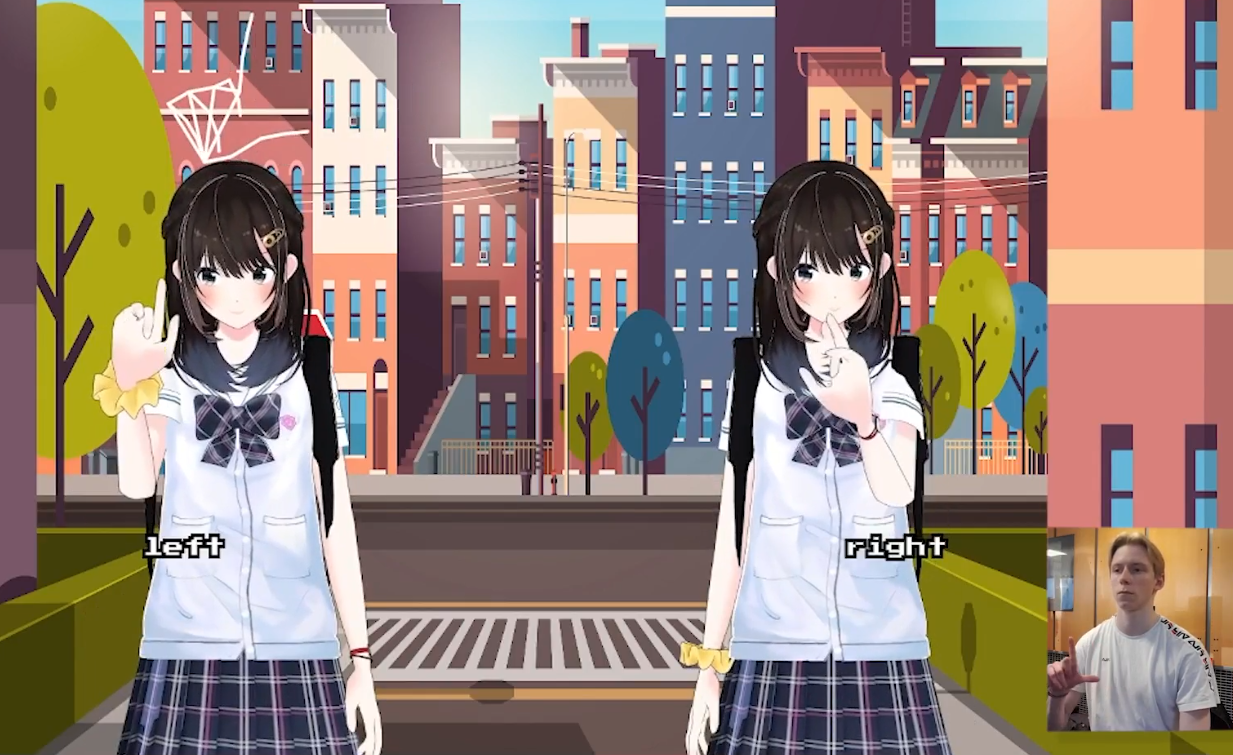
\includegraphics[]{AdrLfv_master_thesis/images/sleg_left_right.png}
    \caption{Choice to go left or right in the sign language learning game.}
    \label{fig:sleg_left_right}
\end{figure}

3D avatars are the models for all the characters. Their limbs (including fingers) are animated. Only the character Aria (the hero's friend) is performing the sign tutorials.
The camera captures the signs, and AI in the back end guesses them. Dialogue lines appear during the adventure to guide and discuss with the player. The user must make the "ok" sign to scroll the text with his hand.



\section{General Architecture}

\subsection{The Sign Language Video Game in GOSAI}

The application is connected to the get\_sign and SLR drivers of GOSAI to estimate the sign of a person in front of the mirror. The socket.io then transmits the data to the engine.js, which runs the game, considering the user's movements (see \ref{fig:sleg_architecture}).

\begin{figure}[h]
    \centering
    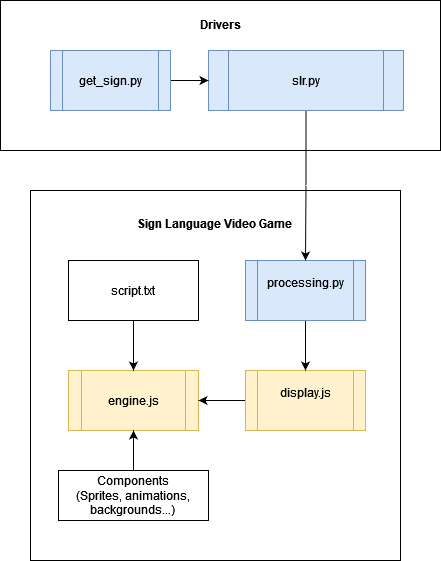
\includegraphics[width=1.6\columnwidth]{AdrLfv_master_thesis/images/sleg_architecture.png}
    \caption{The Sign Language Video Game architecture in GOSAI.}
    \label{fig:sleg_architecture}
\end{figure}

The engine.js accesses the script containing the whole game and the components contained locally (sprites, animations, or backgrounds).

\subsection{Visual Novel Engine}

\subsubsection{Engine implementation}

A visual novel engine had to be implemented to enable the game to function. The P5VN engine is precisely adaptable for the mirror because the engine works with, library already installed on the mirror and used by the majority of its applications.

Previously, p5VN could load and display background, sprites of characters, some text interactive with the mouse click, and menus with multiple buttons.
The engine was running synchronously in a single thread.
Thanks to an important adaptation, the module is now running asynchronously to be compatible with GOSAI. 
The engine loads video animations automatically at launch and can then play them. The user can now interact and select menus thanks to sign language and added many other features.

\subsubsection{Menu}

In a visual novel, the player does not interact directly with the keyboard but must click on menu buttons to make choices. As the user interacts with the mirror only by the estimated pose, the menu system had to be adapted to enable debugging by clicking and making choices with movements.

Each time a menu appears, it takes the form of two or three words aligned and distributed horizontally on the screen. An avatar of Aria (the principal character) appears behind each word to demonstrate the sign related to this word (see \ref{fig:sleg_left_right}). The location of the words and the 3D tutorials are spread over the screen's width according to the number of buttons in the displayed menu. 

Aria's avatar animation plays in a loop until the player makes a sign detected by the SLR module and included in the menu. 

\subsubsection{Script}

A script.txt file contains the game script in the application components. It contains a set of commands starting with the \$ symbol telling the game to do a particular action. These commands can be :
\begin{itemize}
    \item \$tag indicating a specific point in the script
    \item \$jump to jump to a tag
    \item \$defineC to define a character (name, sprite address, text color)
    \item \$defineImg to define an image
    \item \$bg to display a background
    \item \$show to display a character
    \item \$addAnimation to play an animation to a character
    \item \$setSprite to display the sprite of a character
    \item \$menu to create a new menu
    \item \$hide to hide a character
    \item \$setvar to set a variable to a value
    \item \$if to manage if then else commands
\end{itemize}

All the loading of sprites, animations, playback, and display are now managed automatically at startup in asynchronous instead of being set manually in the script or the code as before. The engine was running in synchronous mode at the beginning. The game starts on a loading time at startup corresponding to the loading of sprites and animation videos in the memory of GOSAI. This loading allows the game to play each animation instantly. The game directs the chosen path toward the continuity of the chosen branch. The player can choose different paths to finish the game.

\subsection{Animations}

A module was implemented on the mirror to create accurate custom 3D animations for the animated sign language tutorials. The program allows one to control an avatar in 3D through pose estimation and then record the movements produced or a video of the animation.

An application to control an avatar remotely has been developed on the augmented mirror thanks to the estimation pose. The avatar can track and copy the position of the user's limbs accurately (see \ref{fig:aria_v1}). The created application is now a free demonstration on the mirror. It also allowed the creation of all the 3D character animations on the sign language learning game.

\begin{figure}[h]
    \centering
    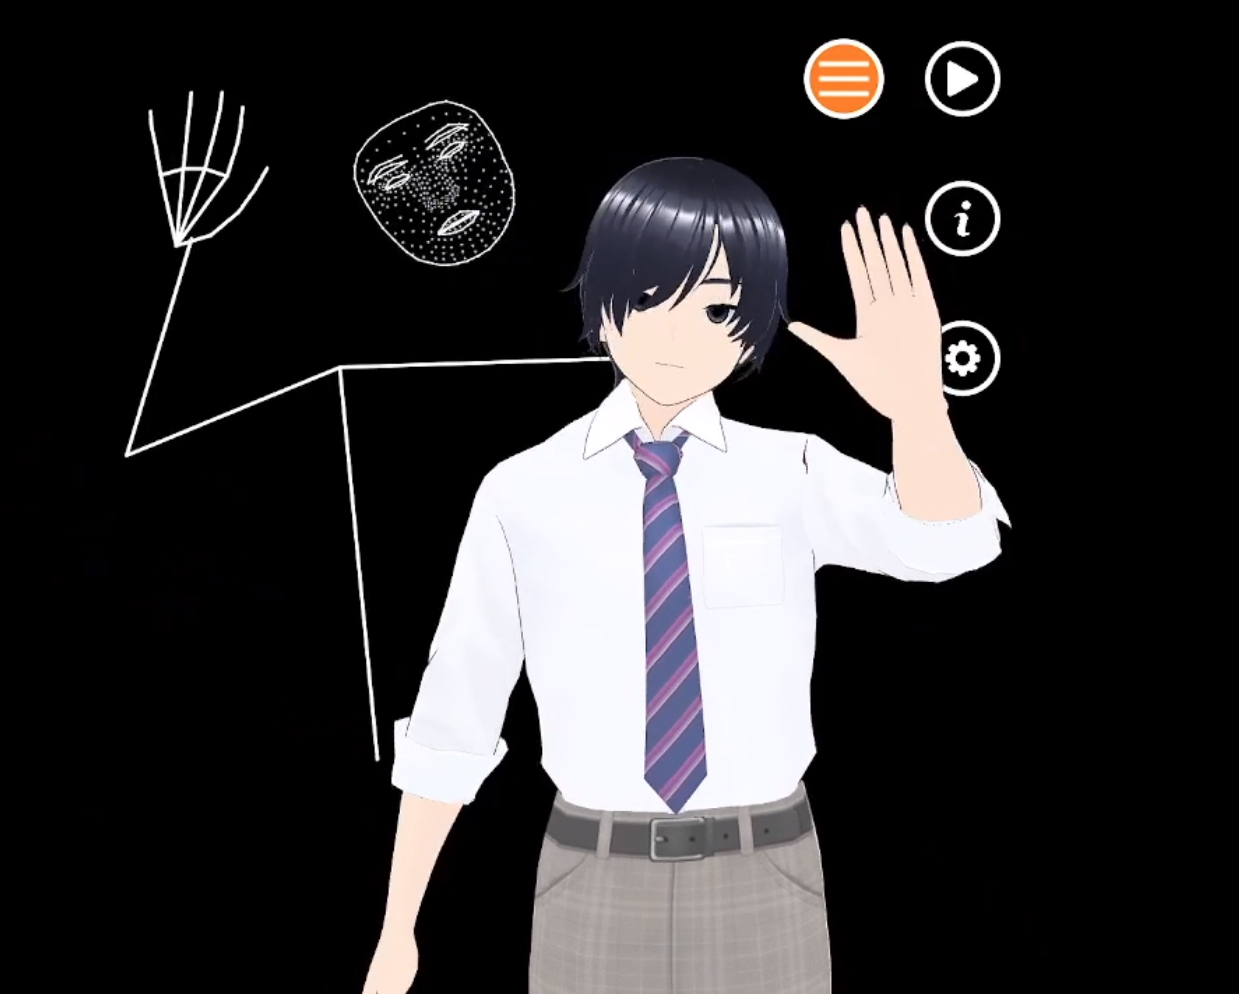
\includegraphics[width=1.6\columnwidth]{AdrLfv_master_thesis/images/aria_v1.png}
    \caption{The first version of the Augmented Reality Interactive Avatar (ARIA).}
    \label{fig:aria_v1}
\end{figure}

\subsubsection{Esla}

The Educative Sign Language Avatar (ESLA) is a 3-dimensional avatar controllable in a GOSAI application following the estimated MediaPipe pose. 

\begin{figure}[h]
    \centering
    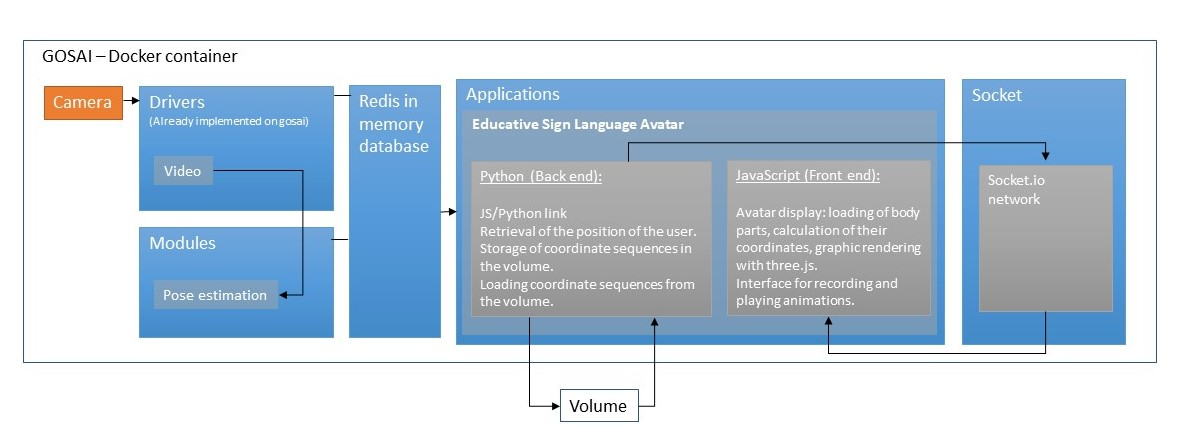
\includegraphics[width=2.25\columnwidth]{AdrLfv_master_thesis/images/esla_architecture.jpg}
    \caption{ESLA architecture on GOSAI.}
    \label{fig:esla_architecture}
\end{figure}

The program uses the driver of the mirror camera, processed by an estimation module (see \ref{fig:esla_architecture}). The Redis database then transmits the data to other modules of the back end in Python. The front end, written in Javascript, manages the display, particularly the calculations related to three.js. Its movements copy live those of the user in front of the mirror \cite{esla}. This version was the first version of the interactive avatar on the augmented mirror.


\begin{figure}[h]
    \centering
    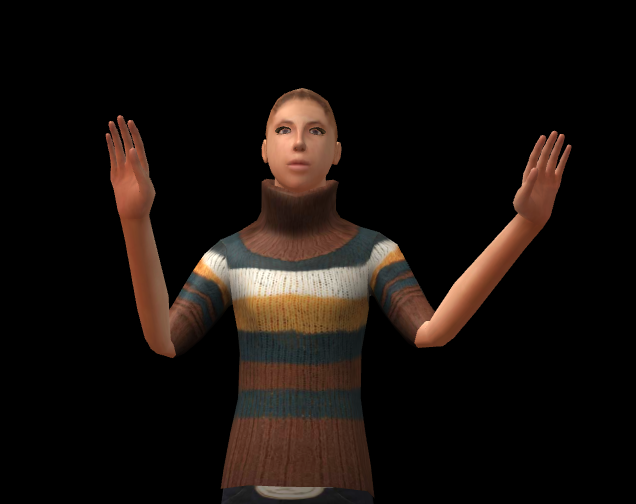
\includegraphics[width=1.4\columnwidth]{AdrLfv_master_thesis/images/esla.png}
    \caption{The Educative Sign Language Avatar (ESLA).}
    \label{fig:esla}
\end{figure}


An animated 3D character appears on top of the scenery at the launch of the application (see \ref{fig:esla}). Its animation is made possible by playing features using MediaPipe and OpenCV. The program can retrieve the coordinates of a user's position in real-time. These coordinates are processed, and the avatar copies the movements thanks to Animation Retargeting, a video game animation technique to map movements on 3D objects.

The program retrieves the links between each point of the pose provided by MediaPipe, and Three.js calculates and displays the 3D part. 

Three.js entirely manages the loading of the character, its display, its animation, the rendering, the light, and the camera.

Three.js uses a pivot system with matrixes and quaternions. However, some functions to transfer rotations from one base to
another still need to be included (even though they are very much in demand by the community). Therefore, the entire limb rotation system was implemented by hand.
MediaPipe first retrieves the (real) coordinates of the user. Transformations convert these coordinates into the world base (x-axis to the right, y-axis to the top, z-axis to the camera) of the three.js scene. The program retrieves the coordinates of the top of the spine, the shoulder, and the elbow (see \ref{fig:esla_bones}). It creates two vectors spine/shoulder and shoulder/elbow. The coordinates of these two vectors are then read from the base of the parent of the bone to be rotated (here, the left shoulder). An algorithm then calculates a quaternion containing the rotation data from the first vector to the second.

\begin{figure}[h]
    \centering
    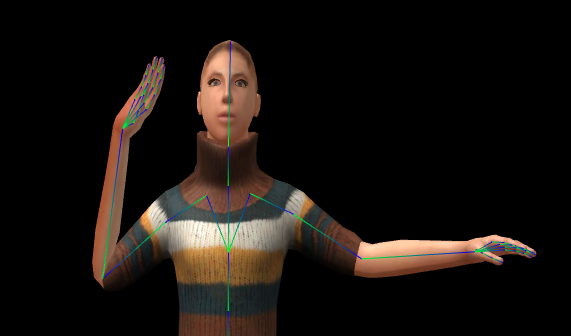
\includegraphics[width=1.6\columnwidth]{AdrLfv_master_thesis/images/esla_bones.png}
    \caption{ESLA's squeletton.}
    \label{fig:esla_bones}
\end{figure}

Three.js then applies this quaternion to the limb, which rotates the same as the user's arm with his shoulder in its local base (see \ref{fig:quaternion_rotations}). This rotation allows precise rotation transfers from one base to another, thus animating all parts of the avatar.

\begin{marginfigure}
    \centering
    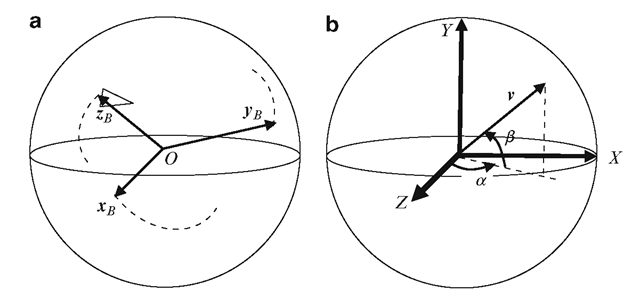
\includegraphics{AdrLfv_master_thesis/images/quaternion_CG.png}
    \caption{Spherical parameterization of rotations: (a) Movement of unit vectors attached to body axes during a rotation of the object. (b) Parametric representation of unit vectors on a sphere \cite{what_when_how}}
    \label{fig:quaternion_rotations}
\end{marginfigure}

Unfortunately, the project lacks much precision in the movements, especially at the level of the fingers, which is very inconvenient for creating accurate tutorials in sign language. Another more efficient solution for creating 3D animations with the estimated pose had to be implemented.

\subsubsection{Kalidokit module implementation}

The creation of an avatar controllable with Mediapipe on the mirror has been by the implementation of the Kalidokit solver. This JS library allows the animation of arms, hands, fingers, face, mouth, eyelids, and pupils of VRM models (Virtual Reality Models). The VRM is based on the standard 3D format glTF2.0 to manage humanoid models. It aims to be particularly expressive. This model has many articulations and can blink and animate its mouth. It is often used in VR games (VR chat) or by Vtubers (entertainment broadcasters who use a virtual avatar).  

The models used in the game come from the site Vroid Hub cite\cite{vroid}. They must respect specific conditions of use: use by a third party, downloadable, use as an avatar, and commercial use by a company. The avatar must also be sober, as it should be a model taking part in a demonstration on the augmented mirror deployed at the De Vinci Innovation Center. The one selected in the demo application allowing to control the avatar in augmented reality is called "papa\_de\_him\_chan". 

The model is easily changeable locally in the application, allowing the user to manipulate different characters. This application makes creating sign language tutorial animations for the learning game possible.

The implementation of Kalidokit on the mirror has been reworked to suit the operation of GOSAI. The joints are set to greater freedom to allow more flexible animations (see \ref{fig:aria_v1}).
Such an application allows recording qualitative signs and poses for the characters and tutorials of the game.

The models used for the characters of Aria, the grandmother, and the salesman were recovered on Vroid Hub and are free to use. The VRM models are mainly adapted for Vtubers, explaining why the characters look childish and look like Japanese anime characters.

\begin{figure}[h]
    \centering
    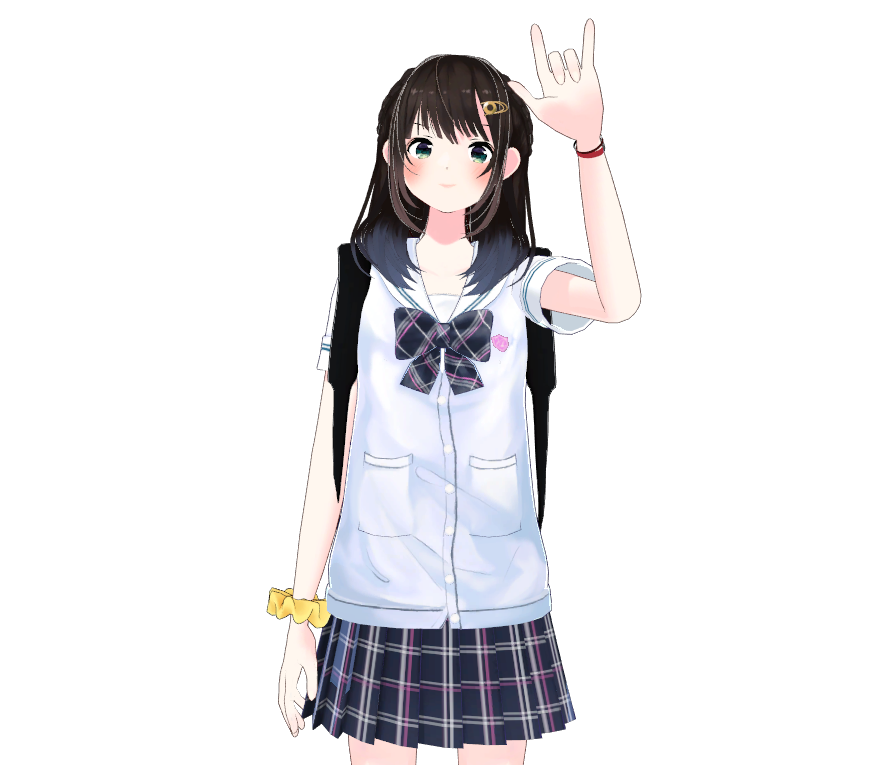
\includegraphics[width=1.4\columnwidth]{AdrLfv_master_thesis/images/iloveyou.png}
    \caption{Aria's character performing the "I love you" sign.}
    \label{fig:iloveyou}
\end{figure}

All the avatars' sprites and 3D video animations were recorded from the "Aria" application on the mirror. These animations include 22 video animations and 14 sprites for the character of Aria in the sign language game (see \ref{fig:iloveyou}).

\section{Sign Language AI}

\subsection{Overview}

A program using computer vision was developed and implemented in the project to enable SLR. This AI allows the recognition of choices in the game thanks to the estimation of the user's pose and the control of the game using commands linked to signs.

Sign language involves using the upper part of the body, such as hand gestures, facial expressions, lip-reading, head nodding, and body postures to disseminate information \cite{adeyanju2021machine}. The model must be able to recognize these different elements.

Many models with sign language recognition already exist. The work done here proposes a model and an easy system of creation, dataset management, training, and visualization of the data.

\subsection{Integration in GOSAI}

The project of creating the SLR AI is apart from GOSAI \cite{slr_mirror}. GOSAI integrates only the weights in a module, making the comparison between a sign made in front of the camera and the values of the weights recorded locally. This architecture means that not all of SLR's AI code is integrated into gosai's code, and only lightweights can be accessed for the comparison.

The video game retrieves the user's coordinates and places them in tensors containing the data of a video of 30 frames. The tensors are then passed to the model, which returns a table of probabilities concerning each action. When the most probable sign is performed for one second, it is transmitted from the SLR module through GOSAI's Redis database to the game engine. The game engine considers a sign to be validated if it is received more than 5 times in a row. This prevents accidental signing.

\subsection{Structure}

The project contains six local modules and a main file that initializes the parameters and launches the different processes. The processes are an optional phase of dataset creation, a tutorial phase that displays the skeleton for data visualization, a preprocessing phase that retrieves the data from the dataset and formats them, a data augmentation module, and a weight calculation and exportation in different file types.

\begin{figure}[h]
    \centering
    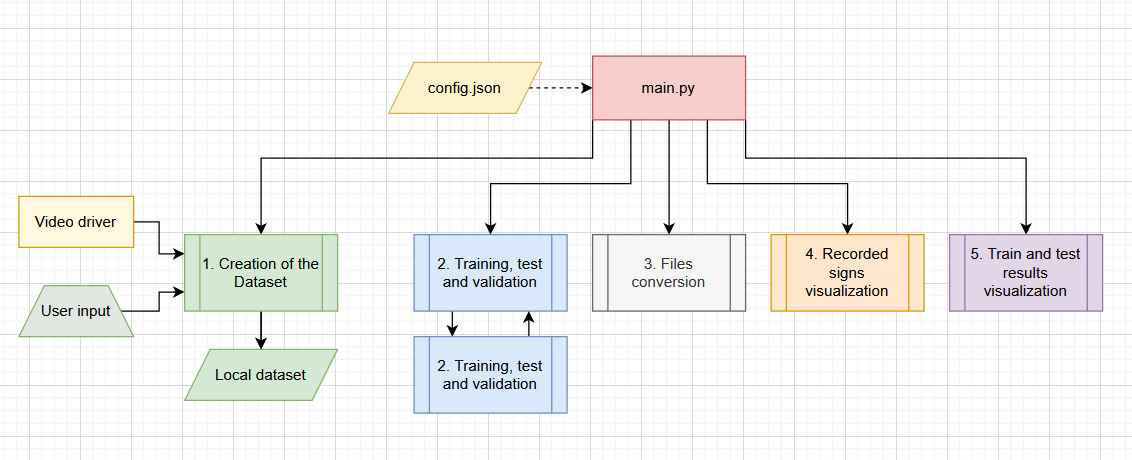
\includegraphics[width=2.2\columnwidth]{AdrLfv_master_thesis/images/SLR_structure.png}
    \caption{Structure of the AI for sign language recognition.}
    \label{fig:SLR_structure}
\end{figure}

The developed AI is a full-fledged project that does not require a goal. It takes five optional steps (see \ref{fig:SLR_structure}). These steps are: the creation of a dataset, the training, test, and validation (with data augmentation or not), the conversion of the created files, the visualization of the recorded signs, and the visualization of the training and test results.

\paragraph{Dataset}

If a movement is included in the known actions but is not present in the files, the creation of the dataset of this movement launches automatically. 

A user creates the database on-live during a dataset recording phase. The data is stored in a folder "MP data" created and separated into three folders: train, valid, and test containing the actions (name of the movement). The recorded sequences are automatically separated between the three folders train (80\% of them), test (10\%), and valid (10\%). The program automatically completes the existing dataset by default according to the number of sequences entered in the configuration file.




Each recorded sign sequence lasts one second, or 30 frames by default. The frames include 58 point coordinates, (or 116 data per frame) after removing 431 points of the face and just Keeping 4. The four kept points are one for the chin, forehead, right, and left cheek. It enables signs using the head to be better detected without recording a large number of points that would not be useful for detection. There are 1600 sequences in all, for a total of 16 different signs, i.e. 100 sequences for each sign (see \ref{fig:slr_dataset}).

%TODO dimension à modifier
\begin{figure}[h]
    \centering
    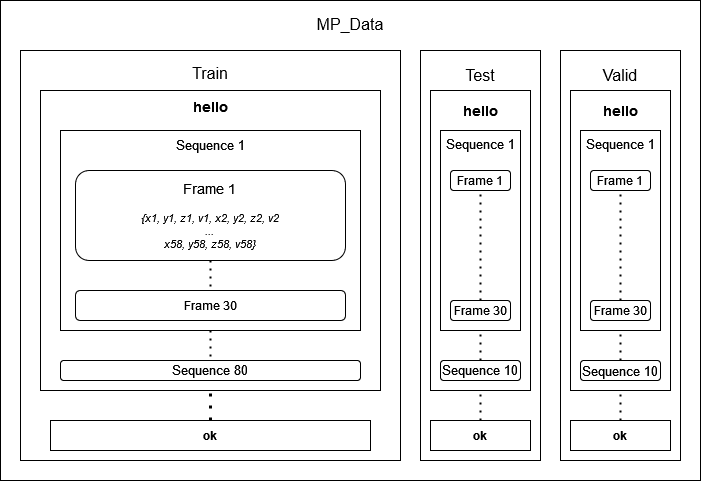
\includegraphics[width=2.2\columnwidth]{AdrLfv_master_thesis/images/Dataset.png}
    \caption{Sign language dataset structure.}
    \label{fig:slr_dataset}
\end{figure}

The program retrieves the coordinates from Mediapipe during the creation of the dataset. If the Intel camera is undetected, the device's webcam record, an Intel real sense, or the default pc webcam. When implemented on another device, such as the interactive mirror, this driver must be modified to match the camera used.

At the start of the dataset creation, the user alternates one second of video recording, then two seconds to reposition in a loop for each sign. He has video feedback on himself to check if he is well-positioned in the plan.

\paragraph{The recorded signs visualization}

The recorded signs visualization module (data\_vis) shows a visualization of every recorded sign (stored in the dataset). This process verifies that the signs have been made and are stored correctly on site.
The program retrieves the coordinates of a person stored in the dataset (for each video), sorts the coordinates of the points of each body part, and finds the different links between each point frame by frame. 

The visualization displays all the links between the points stored in the dataset. The program also displays the action with which the visualization of the sign is associated above the drawn character.

\paragraph{Preprocess}

The preprocessing phase retrieves all the data from the dataset and places them in tensors to provide them to the model.
After creating the preprocess instances (according to their type: train, test, valid), we pass them to the data loader. 

These pass an index to them (concerning a sequence among all the sequences attributed to the type of the preprocess). Their program calculates which action is concerned by the desired sequence and recovers all the coordinates of the frames of this sequence. 
Some papers express that sign language movement is only possible by indicating with lips or facial expressions \cite{cooper2011sign}. Therefore, the dataset should keep some lip coordinates integrated during the preprocessing. For some other papers \cite{dreuw2007speech}, keeping facial and lips expressions is unnecessary to keep these points, which takes much storage for nothing. Here, the preprocess takes into consideration only four coordinates of the face. This selection allows for much faster train loops because all these points are unnecessary.

\paragraph{Data augmentation}

The preprocessing phase optionally calls the data augmentation just after retrieving the data of the concerned sequence. The functionality reviews the data and applies a random horizontal and vertical shift and scale to it. This process artificially increases the number of positions the user can stand.

\paragraph{Model}

The model comprises a bidirectional LTSM, a linear, a dropout, a batchnorm1d, a relu, and another Linear. The model reaches an accuracy of 87\% on the test set and 96\% on the training (see \ref{fig:slr_results}).

\begin{figure}[h]
    \centering
    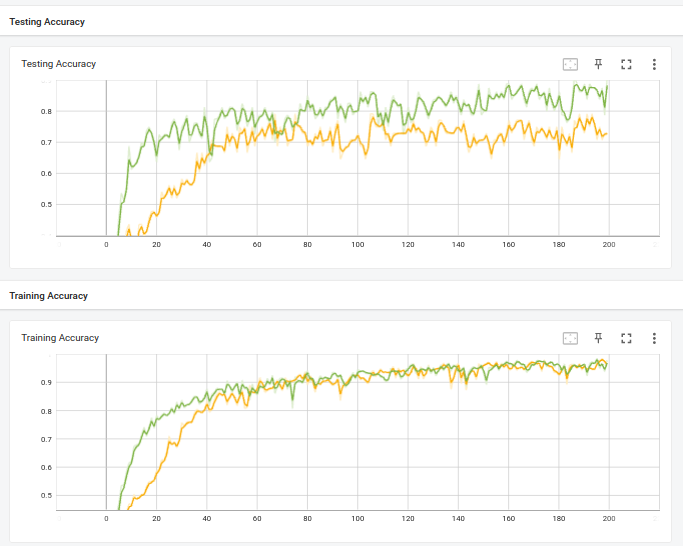
\includegraphics[width=2.2\columnwidth]{AdrLfv_master_thesis/images/slr_results.png}
    \caption{Visualization of testing and training accuracy over 200 epochs. In yellow is the accuracy without data augmentation, and in green with data augmentation.}
    \label{fig:slr_results}
\end{figure}

Recurrent Neural Networks (RNN) allow the processing of temporal sequences (language, videos, numerical data). They keep the memory of past data to predict data sequences shortly. 
LSTM (Long-Short-Term-Memory) and Bidirectional layers are RNNs used in the current model to consider the different coordinates and frames already passed for better performance. The LSTMs are composed of several gates (respectively 3 and 2), which allow one to forget or to selectively memorize the information of the previous temporal sequence in dynamic memory. This RNN is particularly adapted to multiple input dimensions. For example, here, the data is composed of sequences containing frames and coordinates (3 dimensions).
  
The training uses the optimizer AdamW, a stochastic gradient descent method based on adaptive estimation of first-order and second-order moments with an added method to decay weights \cite{loshchilov2017decoupled}. 

The program exports the output models in pth format. Pth is a standard PyTorch convention to save models. They can also be exported to onnx (Open Neural Network Exchange) \cite{onnx}, an open format designed to represent machine learning models.

Onnx extension enables greater interoperability in the AI tool community, allowing many AI frameworks to be more compatible by allowing them to share models. This interoperability allows users to deploy trained models in different software platforms like GOSAI quickly.

Here, the onnx models retrieved from the project output are directly implemented in the SLR module of GOSAI.


\subsection{Configuration}

All the processes mentioned above are optional. The user can enable or disable many project features in the config.json file. 

All the options are: "actions" (all the signs recognized by the AI, "adapt\_for\_mirror" (to transform the coordinates specifically for the augmented mirror), "convert\_files" (to convert the files from pth to onnx), "erase\_dataset" (erasing the dataset before recording a new one), "erase\_runs" (erase the local TensorBoard files), "make\_data\_augmentation", "make\_dataset", "make\_train", "make\_tuto" (visualization of the recorded movements), "nb\_epochs", "nb\_sequences" (total video number the user wants to record for a sign), "sequence\_length" (one video frame number).

The default actions are "nothing", "empty", "ok", "yes", "no", "left", "right", "house", "store", "hello", "goodbye", "television", "leave", "eat", "apple", and "peach". Those are all the signs used inside the SL video game.

The project aims to make it as easy as possible for the user to create weights according to his desired characteristics.

\subsection{Visualization of the results}

TensorBoard is a tool providing visualization solutions to machine learning tests. It allows for tracking and visualizing metrics such as loss and correctness. TensorBoard allows displaying the exported model's graph, histograms of weights, biases or other Tensors, and many other functions.

Just by entering the "make set-up\_tensorboard" function in the terminal (or by doing a "make first\_boot"), the user launches the creation of a local server running on port 6006, retrieving the weights as the model trains. 

A browser page then opens automatically to access the local server address. The user can study a graph of the training and test phase (percentage of success according to the number of epochs) on this page. 

The logs of these results are stored locally. They are accessible on a webpage, and the user can easily compare them. This visualization makes experimentation easier.

\subsection{Limitations}

In the course of numerous experiments, several biases have emerged that directly impact the outcomes of AI. For instance, when there is a significant disparity in body size between the user and the individual who generated the dataset, it often poses a challenge, leading to variations in recognition performance among users with similar or distinct morphologies.

Furthermore, the results of the systematic literature review (SLR) are contingent upon the parameters of Mediapipe, as the AI relies on data obtained from pose estimation for training. The training outcomes indicate that Mediapipe exhibited superior performance in identifying a person's limbs when there was a strong contrast with the background. The selection of the background resulted in a notable performance discrepancy of approximately 15\% between the training and test sets. Mediapipe demonstrated improved capability in detecting the contrast between white skin and a black shirt, and subsequently recognizing instances where a person created the dataset or conducted SLR while wearing such attire.

This contrast renders the SLR more effective for detecting signs produced on the belly, which serves as a plain background devoid of intricate details, compared to signs created in other areas with more background complexity.

\section{Usage scenario}

One of the primary objectives of the augmented mirror is to facilitate interactive learning in augmented reality. It encompasses multiple applications that integrate entertainment and practice functionalities. Users can select and launch specific applications from the mirror's menu. In the context of the sign language game application, users engage with Aria's instructions to embark on an adventure. This game is particularly designed to foster practice and engagement among children.

The augmented mirror eliminates the need for additional equipment, although it requires a sufficient amount of space for optimal usage. Users should be able to stand two meters away from the device and freely execute various movements without any disturbances. It is important to note that the mirror is not suitable for use in dimly lit environments. Adequate lighting conditions are necessary for the camera to accurately detect the user's movements.

\section{User study}

\subsection{Set Up}

As the sign language learning game primarily targets young users, this study focuses on a sample of 12 individuals aged between 18 and 25 years old.

Six participants engage with a selection of video sign language tutorials available on the "pocket sign" application. The tutorials encompass signs that align with the paths taken in the game, such as navigating through the house ("ok," "yes," "left," "right," "house," "store," "hello," "goodbye," "television," "leave," "eat") or the store ("ok," "yes," "no," "left," "right," "house," "store," "goodbye," "apple," "peach"). These individuals are instructed to advance to the next sign once they believe they have comprehended the currently displayed sign.

On the other hand, six participants interact with the sign language learning game using the mirror interface. Before using the game, they receive an explanation of its principles. Two of these participants navigate through the house scenario, while the remaining four navigate through the store scenario.

Both groups are informed from the outset that they will be assessed on specific signs at the conclusion of the study. The duration of each session, from the beginning to the end, is recorded for both groups.


\subsection{Results}

\paragraph{Sign Language Video Game}

Certain users encountered difficulties associated with inadequate AI recognition. For instance, one user required 8 minutes and 25 seconds to complete the game, significantly longer than the average completion time of 4 minutes and 44 seconds. This discrepancy can be attributed to the substantial height difference between the dataset creator (1.84m) and the user (1.60m), thereby introducing bias into the system.

To assess the users' performance, they were evaluated on a random selection of signs following their gaming session. On average, participants achieved a score of 2.33 out of 4 signs learned. The errors observed can be attributed to various factors. In some instances, the AI prematurely identified a sign before the user had accurately positioned their hands, leading to discrepancies between the expected and detected gestures.

\begin{figure}[h]
    \centering
    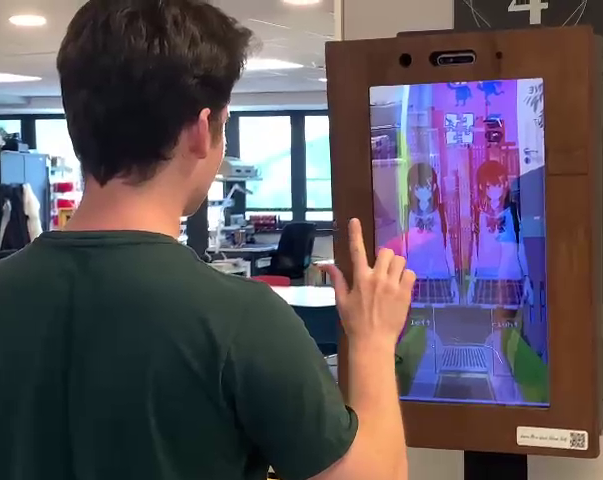
\includegraphics[width=2.2\columnwidth]{AdrLfv_master_thesis/images/slr_game_test.png}
    \caption{Sign Language Video Game user study.}
    \label{fig:slr_game_test}
\end{figure}

Subsequently, users required additional time to observe the signs and make their choices. Another error stemmed from the presence of three simultaneous tutorials (menus with three choices), which hindered users' ability to concentrate on each tutorial, resulting in less efficient sign memorization.

Addressing the issue of AI detection speed can be achieved by increasing the detection threshold value, offering an effective solution.

In conclusion, users were asked to provide their opinions on various aspects of the system using a rating scale of 10. The average motivation to learn sign language through the augmented mirror and video game approach was 7.91/10. Users rated the level of fun in interacting as 8.25/10, ease of understanding the tasks at 7.58/10, practicality of the augmented mirror as a learning method at 8.25/10, and the overall effectiveness of the learning method at 6.41/10. Additionally, users rated the AI's ability to correctly guess signs at 6.11/10.

Overall feedback indicated that the avatars' excessive finger movements compromised precision. The use of a 2D display on the mirror screen, instead of 3D (see \ref{fig:slr_game_test}), posed challenges in understanding the signs. Some users were deterred by the anime-like appearance of the characters, which dampened their enthusiasm for practicing.

A few users forgot the "ok" sign to skip dialogues during the game, despite it being shown twice at the beginning. This forgetfulness hindered their progress and required external intervention for sign reminders. One user faced learning difficulties due to perceived ambiguity in the avatar's movements. However, interacting with a real person facilitated more effective learning. Users strongly criticized the AI's lack of accuracy, rating it at 6.11/10.

The 3D animated tutorials garnered positive feedback and were considered more engaging than simple video tutorials. Users expressed satisfaction with using the game on an augmented mirror, deeming the mirror's interface mainstream and easily integrable into a living room setting.

% \paragraph{Videos}

% \textit{POTENTIAL USER STUDY ABOUT LEARNING WITH VIDEO TUTORIALS}

\section{Discussions}

The Sign Language Game effectively stimulates visual, verbal, and kinesthetic intelligence among its users. Visual intelligence encompasses the ability to mentally construct images and accurately perceive the three-dimensional visual world. By engaging with 3D sign language tutorials and deciphering the diverse movements and limb positions of the avatars, users' visual intelligence is stimulated. They must perceive and mentally project the identified signs before reproducing them.

Verbal intelligence pertains to rapid reading, speaking, and the capacity to articulate mental concepts into words. Connecting visual images to corresponding words within the project enhances users' fluency in expressing themselves and linking mental ideas to gestures.

Kinesthetic intelligence involves the refined utilization of one's body, expressing oneself through movement, and precise control over bodily motions. The project's gamified approach stimulates this form of intelligence as users must translate mental images of body positions and movements into real-world actions.

The simultaneous stimulation of these three intelligences, coupled with the motivational aspects of gamification, enhances information retention. Users retain sign language gestures more effectively through the combination of visual observation, mental projection, and physical execution in space. Studies have demonstrated the influential impact of non-verbal behaviors, such as gestures, on comprehension and memory in communication \cite{kelly1999offering}.

\section{Conclusion}

\subsection{Playful Learning and ASL}


Playful learning and gamification are pedagogical approaches that leverage elements of play to enhance the acquisition of knowledge. These approaches are frequently employed in educational contexts, including the use of video games, to facilitate the teaching of practical skills such as sign language. By integrating augmented reality, pose estimation, and artificial intelligence, the Sign Language Video Game offers an immersive and interactive learning experience, enabling learners to practice reproducing signs accurately in real-time.

This approach facilitates learning through immediate feedback, allowing learners to engage in repeated practice sessions at their own pace. Furthermore, the incorporation of cutting-edge technologies in the game design tends to generate curiosity and captivate learners, thereby fostering increased motivation and perseverance in the acquisition of sign language skills.

\subsection{Limitations}

The findings from the user studies highlight several limitations within the project.

One limitation pertains to the size discrepancy between the individual who created the dataset and potential users with varying heights. While the accuracy is high for the dataset creator, it diminishes for users with different morphologies. To address this issue, one potential solution is to introduce random compression of coordinates along the horizontal and vertical axes during data augmentation or to include individuals of diverse sizes during dataset registration.

The dataset utilized in the project is relatively small, exhibiting limited noise, slight variations, and minimal mixing. Although the model demonstrates moderate efficiency, even when trained on multiple distinct signs, its accuracy would further decline with dataset expansion. Therefore, the model should be reworked in the future. The implementation of transformers could prove beneficial, enhancing performance. Transformers have proven successful in various domains such as image processing, biological sequence analysis, and video understanding.

Another area for improvement concerns the clarity of avatars in sign language tutorials, which can sometimes be challenging. The pivot angles of the avatar's bones are constrained to prevent glitches and ragdoll-like movements. Consequently, capturing clear signs, particularly at the finger level, can be difficult. As a result, users must imitate and learn from an inaccurate model. To address this issue, slight modifications can be made to widen the allowable angles of the avatar's bones, thereby enhancing precision.

\subsection{Future Works}

The current game is suitable for direct practice. However, the learning system is too simple because users can afford to copy the sign without actually learning it. It would be necessary to add an evaluation dimension with signs that come up in the potential choices without giving the tutorials every time. Thus the user will have to force himself to remember and learn better by repetition.

\paragraph{Current work}

This dimension of training is already present in another mirror-based application, resembling sign language training. The application comprises consecutive viewings of sign language tutorial videos, practice sessions, and a correction phase. During the correction phase, frozen Mediapipe bones and points, forming a skeletal structure, manifest on the mirror and perform the initial stage of a sign.

The user is provided with a Mediapipe skeleton displayed on the mirror, which tracks their movements. When the user overlays their skeleton onto the model's skeleton, the model's skeleton undergoes slight adjustments to present the subsequent frame of the recorded sign movement. Subsequently, the user must align their skeleton with the second frame until they validate the 30 frames constituting a sign. Specifically, the person needs to align certain points of their body, particularly their hands and fingers. These corrections facilitate precise learning of the executed sign. The training then proceeds to a tutorial of another sign.

Implementing the correction phase of this training within the sign language game would yield significant benefits. The corrections enhance the user's sign retention by requiring them to repeatedly perform the signs while focusing on the positioning of each finger. The clear demonstrations of the signs enable the user to visualize the accurate spatial positioning they need to adopt. Consequently, this implementation would address some of the current issues in the game. Although the correction phase is presently excluded due to its disruption of the game's flow, integrating it at the game's conclusion as a reminder of the learned signs would serve as an effective learning method.